\documentclass[14pt,a4paper,oneside,fleqn]{tmarticle}
\usepackage[]{lipsum}
\usepackage[spanish]{babel}
\usepackage[utf8]{inputenc}
\usepackage[scaled=0.85]{beramono}
\usepackage[T1]{fontenc}
\usepackage[backend=biber,style=numeric,sorting=none]{biblatex}
\usepackage[toc,section=section]{glossaries}
\makeglossaries{}
\newglossaryentry{placeholder} {
  name=placeholder,
  description={placeholder}
}
\usepackage{bibentry}
\nobibliography{bibliography.bib}
\addbibresource{bibliography.bib}
\bibstyle{plain}
\usepackage[]{paralist}
\renewcommand{\familydefault}{\sfdefault}
\usepackage{titlesec}
\usepackage[]{rotating}
\usepackage[]{fancyhdr}
\usepackage[a4paper,width=150mm,top=25mm,bottom=25mm,bindingoffset=6mm]{geometry}
\usepackage[]{xcolor,colortbl}
\graphicspath{{img/}{../img/}}
\usepackage{pdfpages}
\usepackage[]{svg}
\usepackage[]{amsmath}
\usepackage{pgfgantt}
\usepackage[]{amssymb}
\DeclareTextCommand{\nobreakspace}{T1}{\leavevmode\nobreak\ }
\titleclass{\subsubsubsection}{straight}[\subsection]

\newcounter{subsubsubsection}[subsubsection]
\renewcommand\thesubsubsubsection{\thesubsubsection.\arabic{subsubsubsection}}
\renewcommand\theparagraph{\thesubsubsubsection.\arabic{paragraph}} % optional; useful if paragraphs are to be numbered

\titleformat{\subsubsubsection}
  {\normalfont\normalsize\bfseries}{\thesubsubsubsection}{1em}{}
\titlespacing*{\subsubsubsection}
{0pt}{3.25ex plus 1ex minus .2ex}{1.5ex plus .2ex}

\makeatletter
\renewcommand\paragraph{\@startsection{paragraph}{5}{\z@}%
  {3.25ex \@plus1ex \@minus.2ex}%
  {-1em}%
  {\normalfont\normalsize\bfseries}}
\renewcommand\subparagraph{\@startsection{subparagraph}{6}{\parindent}%
  {3.25ex \@plus1ex \@minus.2ex}%
  {-1em}%
  {\normalfont\normalsize\bfseries}}
\def\toclevel@subsubsubsection{4}
\def\toclevel@paragraph{5}
\def\toclevel@paragraph{6}
\def\l@subsubsubsection{\@dottedtocline{4}{7em}{4em}}
\def\l@paragraph{\@dottedtocline{5}{10em}{5em}}
\def\l@subparagraph{\@dottedtocline{6}{14em}{6em}}
\makeatother
\setcounter{secnumdepth}{4}
\setcounter{tocdepth}{4}
\begin{document}
\pagestyle{fancy}
\begin{titlepage}
	\centering
        
\includegraphics[scale=0.75]{puiglogo.png}\par\vspace{1,5cm}
            {\huge\bfseries Análisis de datos con Apache Cassandra y Python\par}
	\vspace{0.5cm}
	    {\scshape\Large Memoria\par}
	\vspace{0.5cm}
	    {\scshape\Large CFGS Desarrollo de Aplicaciones Multiplataforma\par}
	\vspace{6.0cm}
  \hfill{\Large\textbf{Enrique Villarreal}}\par
  \vspace{0.1cm}
  \hfill{\Large\textbf{Adrián Asensio}}\par  
        \vspace{1.5cm}
            \hfill{\large Curso \textbf{2016-2017}\par}
            \hfill{\large\today\par}
         \vspace{2cm}
         \begin{flushright}

        
\includegraphics[scale=0.75]{creativecommons.png}\par\vspace{0.05cm}

           Esta obra está sujeta a una licencia de Reconocimiento-NoComercial-SinObraDerivada 3.0 España de Creative Commons
         \end{flushright}
        \vfill
\end{titlepage}
\thispagestyle{empty}
\textbf{Resumen}
\vspace{0.5cm}

Nullam eu ante vel est convallis dignissim.  Fusce suscipit, wisi nec facilisis facilisis, est dui fermentum leo, quis tempor ligula erat quis odio.  Nunc porta vulputate tellus.  Nunc rutrum turpis sed pede.  Sed bibendum.  Aliquam posuere.  Nunc aliquet, augue nec adipiscing interdum, lacus tellus malesuada massa, quis varius mi purus non odio.  Pellentesque condimentum, magna ut suscipit hendrerit, ipsum augue ornare nulla, non luctus diam neque sit amet urna.  Curabitur vulputate vestibulum lorem.  Fusce sagittis, libero non molestie mollis, magna orci ultrices dolor, at vulputate neque nulla lacinia eros.  Sed id ligula quis est convallis tempor.  Curabitur lacinia pulvinar nibh.  Nam a sapien.

\vspace{0.5cm}
\textbf{Palabras clave: } big data, data science, nosql, cassandra, python

\clearpage
\textbf{Abstract}
\vspace{0.5cm}

Nullam eu ante vel est convallis dignissim.  Fusce suscipit, wisi nec facilisis facilisis, est dui fermentum leo, quis tempor ligula erat quis odio.  Nunc porta vulputate tellus.  Nunc rutrum turpis sed pede.  Sed bibendum.  Aliquam posuere.  Nunc aliquet, augue nec adipiscing interdum, lacus tellus malesuada massa, quis varius mi purus non odio.  Pellentesque condimentum, magna ut suscipit hendrerit, ipsum augue ornare nulla, non luctus diam neque sit amet urna.  Curabitur vulputate vestibulum lorem.  Fusce sagittis, libero non molestie mollis, magna orci ultrices dolor, at vulputate neque nulla lacinia eros.  Sed id ligula quis est convallis tempor.  Curabitur lacinia pulvinar nibh.  Nam a sapien.

\vspace{0.5cm}
\textbf{Keywords: } big data, data science, nosql, cassandra, python

\clearpage
\thispagestyle{empty}
\tableofcontents
\clearpage
\thispagestyle{empty}
\listoffigures
\clearpage
\pagenumbering{arabic}

\section{Introducción}
\label{sec:aim}

\subsection{Contexto y justificación}
\label{subsec:context}

Las bases de datos relacionales llevan con nosotros desde hace más de 40 años.
Están basadas en el modelo relacional (\cite{Codd:1970:RMD:362384.362685}), en el que los datos se representan en tuplas, agrupadas en
relaciones, que por lo general, representan entidades. Por tanto, almacenan
\textbf{datos estructurados}, y resultan ideales en situaciones en las cuales el
modelo de los datos está rígidamente definido.

De todas maneras, la mayor parte de la información que se genera a
diario en Internet (pista: mucha), no se ajusta a niguna estructura, y
por tanto, no puede ser almacenada tal cual en sistemas con esquemas definidos.
En respuesta a ello, y al rápido aumento en la cantidad de datos a procesar,
surgieron las \textbf{bases de datos NoSQL}. Al no usar el tradicional modelo
relacional, éstas resultan mucho más adecuadas para manejar datos sin ningún
tipo de organización o estructura. 

Otro de los conceptos al que va enfocado el proyecto es el de ciencia de los
datos, posiblemente el último ``no va más'' en el mercado. Hasta ha sido
clasificado por Glassdoor como el mejor trabajo en América a inicios de 2016
\footnote{\url{https://www.glassdoor.com/blog/25-jobs-america-2016/}}. Uno de
los motivos por los cuales decidimos explorar éste concepto en el proyecto es el
hecho de que aunque lleva ya tiempo establecido, aún sigue sin un currículo
estandarizado, o una definición concreta a la que acogerse.

\subsection{Objetivos}
\label{subsec:objectives}

Los objetivos principales del proyecto son:

\begin{itemize}
    \item Estudiar y conocer las bases de datos NoSQL, en concreto Apache Cassandra
      \begin{itemize}
      \item Identificar los usos ideales para su uso.
      \end{itemize}
    \item Entender el diseño y modelado de datos en Apache Cassandra.
    \item Utilizar la \emph{API Streaming} de Twitter para almacenar twits que
      hagan referencia a un \emph{hashtag}.
    \item Entender y familiarizarse con el flujo de trabajo del científico de datos.
      \begin{itemize}
      \item Realizar análisis de sentimiento de los twits obtenidos mediante Python.
      \end{itemize}
\end{itemize}

\subsection{Metodología}
\label{subsec:metodologia}

El proyecto se dividirá en dos partes: la primera consistirá en un estudio de
las bases de datos NoSQL, concretamente Apache Cassandra, y una
comparativa con bases de datos relacionales. Además, exploraremos el concepto de
\emph{ciencia de los datos}, una nueva profesión que combina diferentes
disciplinas, desde la programación hasta las matemáticas y la estadística,
centrada en en la solución de problemas / obtención de conocimiento a partir de
información. 

La segunda parte consistirá en utilizar lo aprendido en la primera parte para
implementar un sistema que aproveche las aptitudes de Cassandra para el
\emph{big data} y el análisis de datos. A ése fin, utilizaremos la API Streaming
de Twitter para obtener twits y almacenarlos en Apache Cassandra, sobre los
cuales luego utilizaremos Python para realizar análisis de sentimiento sobre los
twits.

\subsection{Características técnicas}
\label{subsec:planificació}

Aquí se detallan las tecnologías y herramientas que se prevé
utilizar durante el proyecto:

\begin{itemize}
    \item \textbf{Documento de la memoria: } \LaTeX
    \item \textbf{SGBD NoSQL: } Apache Cassandra
    \item \textbf{Lenguaje de programación: } Python 
    \item \textbf{Librerías: } 
      \begin{itemize}
      \item Datastax Cassandra driver for Python
      \item Tweepy
      \item Pandas
      \item Natural Language Toolkit (NLTK)
      \end{itemize}
    \item \textbf{Presentación: } Reveal.js
    \item \textbf{Aplicaciones auxiliares: } 
      \begin{itemize}
        \item Jupyter Notebook
      \end{itemize}
\end{itemize}

\textbf{Nota:} Se irá actualizando ésta lista a medida que se van descubriendo
nuevas herramientas y librerías.


\subsection{Planificación del proyecto}
\label{subsec:planificació}

\subsubsection{Lista de tareas}
\label{subsubsec:tasklist}

\begin{table}[!htb]
\centering
\begin{tabular}{l|l|l|l|l|l|}
\hline
\multicolumn{5}{|c|}{Tarea}                                                                                                       & Predecesora \\ \hline
\multicolumn{2}{|l|}{\textbf{1}} & \multicolumn{3}{l|}{\textbf{Redactar  estudio}}                                                &             \\ \hline
              & 1.1              & \multicolumn{3}{l|}{Describir brevemente las bases de datos NoSQL}                             &             \\ \cline{2-6} 
              & 1.2              & \multicolumn{3}{l|}{Estudiar Apache Cassandra: su modelo de datos, y sus casos de uso ideales} & 1.1         \\ \cline{2-6} 
              & 1.3              & \multicolumn{3}{l|}{Realizar una comparativa con las bases de datos relacionales}              & 1.2         \\ \cline{2-6} 
              & 1.4              & \multicolumn{3}{l|}{Definir el concepto de ciencia de los datos}                               &             \\ \cline{2-6} 
              & 1.5              & \multicolumn{3}{l|}{Entender la metodología del científico de datos}                           & 1.4        \\ \hline

\multicolumn{2}{|l|}{\textbf{2}} & \multicolumn{3}{l|}{\textbf{Implementación del proyecto}}                                      & \textbf{1}  \\ \hline
              & 2.1              & \multicolumn{3}{l|}{Estudio de algoritmos de clasificado y selección del mismo.}               &             \\ \cline{2-6} 
              & 2.2              & \multicolumn{3}{l|}{Diseño e implementación de la base de datos}                               & 2.1         \\ \cline{2-6} 
              & 2.3              & \multicolumn{3}{l|}{Introducción a los algoritmos de clasificado}                              & 2.2         \\ \cline{2-6} 
              & 2.4              & \multicolumn{3}{l|}{Implementación del programa para popular la base de datos}                 & 2.3         \\ \cline{2-6} 
              & 2.5              & \multicolumn{3}{l|}{Análisis de los datos}                                                     & 2.4         \\ \hline
\multicolumn{2}{|l|}{\textbf{2}} & \multicolumn{3}{l|}{\textbf{Redacción de la memoria}}                                          &             \\ \hline
\end{tabular}
\end{table}

\subsubsection{Diagrama Gantt}
\label{subsubsec:tasklist}

\vspace{0.45cm}
\hspace*{-1.2in}
\begin{ganttchart} [
  hgrid,
  vgrid,
  x unit = 4mm,
  time slot format = isodate,
  ]{2017-3-7}{2017-4-8}
  \gantttitlecalendar{year, month, day}\\

  \ganttbar{Introducción}{2017-3-7}{2017-3-15}\\
  \ganttlinkedbar{Apache Cassandra}{2017-3-15}{2017-4-2}\\
  \ganttlinkedbar{Comparativa}{2017-4-2}{2017-4-4}\\ 
  \ganttlink{elem0}{elem1}
  \ganttlink{elem1}{elem2}

  \ganttgroup{Ciencia de los datos}{2017-3-7}{2017-4-7}\\
  \ganttbar[name=dataIntro]{Introducción}{2017-3-7}{2017-3-15}\\
  \ganttbar[name=flujo]{Flujo de trabajo}{2017-3-15}{2017-3-22}\\
  \ganttbar[name=class]{Algoritmos de clasificado}{2017-3-22}{2017-4-7}\\

  \ganttlink{dataIntro}{flujo}
  \ganttlink{flujo}{class}
  
  \ganttmilestone{Entrega estudio}{2017-4-7}
\end{ganttchart}

\vspace{1cm}
\hspace*{-1.3in}
\begin{tikzpicture}[y = 5mm]
\begin{ganttchart} [
  hgrid,
  vgrid,
  x unit = 4mm,
  time slot format = isodate,
  bar top shift=-0.1]{2017-4-8}{2017-5-12}
  \gantttitlecalendar{year, month, day}\\

  \ganttbar[name=dbDesign]{Diseño base de datos}{2017-4-8}{2017-4-12}\\

  \ganttgroup[name=impl]{Implementación}{2017-4-12}{2017-4-25}\\
  \ganttbar[name=algo]{Selección de algoritmo}{2017-4-12}{2017-4-16}\\
  \ganttbar[name=impl2]{Implementación prog.}{2017-4-16}{2017-4-25}\\
  \ganttbar[name=unitTest]{Pruebas unitarias}{2017-4-18}{2017-4-25}\\

  \ganttlinkedbar[name=analisis]{Análisis de los datos}{2017-4-27}{2017-5-11}\\

  \ganttlink{dbDesign}{impl}
  \ganttlink{algo}{impl2}
  \ganttlink{impl}{analisis}

  \ganttmilestone{Entrega implementación}{2017-5-12}
\end{ganttchart}
\end{tikzpicture}

\begin{center}
  \textbf{Nota: } El análisis de datos es un proceso largamente iterativo, la
  longitud en el diagrama es orientativa.
\end{center}

\vspace{1cm}
\hspace*{-1.3in}
\begin{tikzpicture}[y = 5mm]
\begin{ganttchart} [
  hgrid,
  vgrid,
  x unit = 4mm,
  time slot format = isodate,
  bar top shift=-0.1]{2017-5-12}{2017-6-3}
  \gantttitlecalendar{year, month, day}\\
  \ganttbar[name=code]{Documentación del código}{2017-5-12}{2017-6-1}\\

  \ganttmilestone{Entrega del producto}{2017-6-3}
\end{ganttchart}
\end{tikzpicture}

\subsection{Descripción de los capítulos}
\label{subsec:chaps}

\begin{enumerate}
  \item \textbf{Estado del arte: }
    \begin{enumerate}
      \item \textbf{NoSQL y Apache Cassandra: } En esta sección estudiaremos
        brevemente las bases de datos NoSQL, en concreto Apache Cassandra.
        Trataremos de entenderlas, e identificar aquellas situaciones en las que
        es ideal utilizarlas.
      \item \textbf{Ciencia de los datos: } Aquí introduciremos y exploraremos el
        concepto de ciencia de los datos. Intentaremos desentrañar a qué se refiere
        exactamente, con qué herramientas se trabaja, y con qué objetivos.
        Haremos énfasis en el flujo de trabajo del científico de los datos, es
        decir, la metodología estándar en un proyecto de éstas características.
    \end{enumerate}

  \item \textbf{Implementación: } En ésta sección documentaremos
    la implementación de la base de datos, y el análisis de los twits, razonando
    cada decisión técnica tomada a lo largo del proceso.
  \item \textbf{Conclusiones: } A ser redactada en la última entrega de la
    memoria, en ésta sección daremos nuestras opiniones sobre nuestro
    aprendizaje de la temática del proyecto, y el proceso de implementación del mismo.
  \item \textbf{Anexo: } En éste capítulo se incluirán guías y descripciones
    varias como la preparación del entorno de desarrollo, y otras.
\end{enumerate}

\subsection{Formato de éste documento}
\label{subsec:format}

En el documento, se utilizarán las siguientes convenciones de formato:

    \begin{TMterminal}{}{}{Bloque de comandos}
      comandos a ser introducidos por el usuario en un intérprete de comandos
    \end{TMterminal}

    \vspace{0.2cm}

    \begin{TMcode}{Python}{}{Bloque de código}
      for i in range(1,10):
          print("Código fuente")
    \end{TMcode}

    \begin{TMbulletin}{normal}{Aviso}
      Información a tener en cuenta.
    \end{TMbulletin}

    \begin{TMbulletin}{warning}{$¡$Aviso importante!}
      Información importante a tener en cuenta.
    \end{TMbulletin}

    \begin{TMbulletin}{critical}{$¡$Aviso muy importante!}
      Información muy importante a tener en cuenta.
    \end{TMbulletin}
\clearpage

% \chapter[Estado del arte]{Estado del arte, requisitos y arquitectura}
\label{sec:state_of_art}

\section{Virtualización de servidores}
\label{subsec:virt_servers}

Como ya dije antes, la virtualización aplicada a servidores no es nada que haya surgido los últimos años. Pero cuando IBM comenzó a trabajar con los primeros \emph{mainframes} concurrentes, su propósito era meramente ofrecer a sus usuarios una manera de trabajar al mismo tiempo en un mundo que, en aquellos tiempos, era puramente secuencial.

Hoy en día la virtualización ha ido evolucionando gradualmente, resultando en diferentes técnicas y métodos que permiten sustituir de manera eficaz y flexible las máquinas físicas. Cada método funciona de una manera diferente, con sus ventajas y desventajas, que iré explorando brevemente en las siguientes secciones:

\subsection{Cómo opera el instituto actualmente}
\label{subsubsec:virt_des}

Antes de discutir los pros y los contras de los diferentes métodos de virtualizacion, veamos cómo se ofrecen los servicios actualmente: en una máquina personalizada con las siguientes características:

\begin{itemize}
    \item \textbf{CPU:\@ }Intel Xeon E-1220 @ 3.10 GHz
    \item \textbf{RAM:\@ }8 GB
\end{itemize}

Considerando los servicios ofrecidos (Un par de servidores web con la página web del centro y un Owncloud, y un servidor DHCP.), ésta máquina está lo suficientemente preparada para dichos servicios, pero opino que se pueden ofrecer de manera más eficiente. A continuación, listaré los que a mi juicio son los principales detrimentos de éste sistema:

\begin{itemize}
    \item \textbf{Aprovechamiento mínimo de recursos: }Aunque ésto se vea atenuado de cierto modo en este caso, los recursos de una máquina raramente se aprovechan del todo, ya que un servicio no hará uso de todo el hardware disponible.

    \item \textbf{Ningún tipo de aislamiento entre servicios: }Debido a que todos los servicios se están ejecutando en el mismo sistema operativo sin ningún mecanismo de aislamiento, cualquier problema grave en cualquiera de los servicios podría comprometer la disponibilidad de los otros servicios.

    \item \textbf{Costos de expansión: }Expandir ésta arquitectura puede resultar muy costoso, tanto en materia de hardware, electricidad, y acondicionamiento de la sala de servidores.
\end{itemize}

\subsection{Ventajas de la virtualización}
\label{subsec:virt_servers}
 
Incluso si éstos no parecen tan malos, todavía son suficientemente crtíicos para considerar un cambio a un sistema basado en máquinas virtuales. Algunas de las ventajas son:

\begin{itemize}
    \item \textbf{Aislamiento de servicios: }Las máquinas virtuales son, en esencia, ordenadores enteros emulados dentro de una máquina física, así que el resultado es el mismo que antes: Estamos ejecutando cada servicio dentro de su propia máquina. Esto asegura que un servicio que falle no puede tumbar otros servicios, asumiendo que éstos se estén ejecutando en una máquina virtual diferente. 

    \item \textbf{Ahorro: }Ésta tranquilamente podría ser la razón principal. No sólo baja el coste del hardware adicional, pero también resulta en menos mantenimiento, menor coestes eléctricos, y otras tareas relacionadas con el espacio de trabajo.

    \item \textbf{Un ciclo de trabajo más rápido: } Comparad el tiempo que tardáis en crear una nueva máquina virtual, y en preparar un ordenador físico al punto que es sea capaz de ofrecer un servicio. Ésto nos permite usar el sistema de virtualización tanto para servicios en producción, y experimentos y pruebas variadas.

    \item \textbf{Menor tiempo de indisponibilidad: }Combinando técnicas de ahorro de energía y aseguramiento eléctrico como SAIs, y el uso de un sistema de virtualización que lo soporte, las máquinas virtuales pueden ser migradas en caliente entre diferentes hosts, permitiendo la realización de tareas de mantenimiento sin que los usuarios se den cuenta.

    \item \textbf{Recuperación acelerada en caso de desastre: }Las máquinas virtuales pueden ser respaldadas a ficheros, y re-importadas en un servidor diferente en caso de emergencia. Herramientas como oVirt pueden incluso reiniciar máquinas fallidas en otro host diferente si el que previamente virtualizaba la máquina falla.
\end{itemize}

\begin{TMbulletin}{warning}{$¡$Importante!}
  Pese a todo ésto, sigue siendo muy importante el uso de sistemas de alimentación ininterrumpida para asegurar el equipo de red y los ordenadores y minimizar los SPOF.\@
\end{TMbulletin}

\subsection{Métodos de virtualización}
\label{subsubsec:virt_servers}

Después de haberle echado una ojeada a los pros y contras de la virtualización frente al modelo distribuido, veamos de qué maneras podemos crear y utilizar máquinas virtuales:

\subsubsection{Virtualitzación de hardware completa}
\label{subsubsubsec:virt_complete}

La virtualización de hardware completa es un método en el cual la máquina virtual resultante es una simulación entera de todo el hardware de un ordenador físico, incluyendo elementos como el juego de instrucciones de la CPU, interrupciones, y otros elementos que permiten que los programas se ejecuten sobre el \emph{bare metal}.

La virtualización completa en x86 fue inicialmente desarollada por VMware en 1998, mediante técnicas de traducción binaria, y ejecucción directa. Para entender mejor éste aspecto, es necesario conocer un poquito de la arquitectura x86, en concreto los \textbf{anillos de protección} \cite{vmware}: una serie de ``niveles'', que definen y aíslan los privilegios de los que cierto código dispone. Típicamente, las aplicaciones de usuario se ejecutan sobre el nivel 3, el menos privilegiado, y código referente a la gestión de la memoria, o cualquier otras funciones del sistema operativo, en el nivel 0, el más privilegiado.

\clearpage
\begin{figure}[ht]
  \centering
  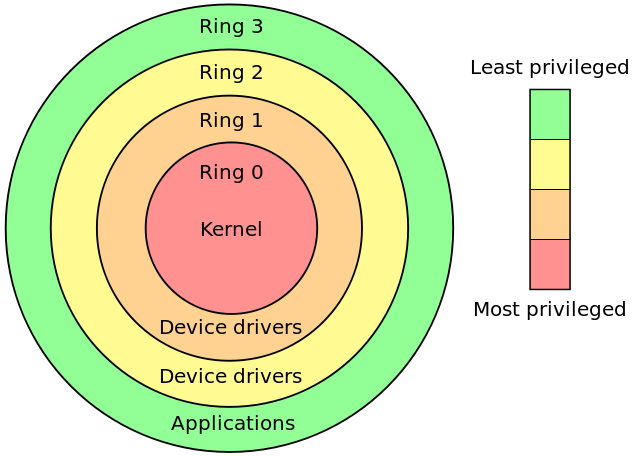
\includegraphics[scale=0.40]{rings.png}
  \caption{\label{fig:label} Anillos de protección, por Hertzsprung en Wikipedia}
\end{figure}
\vspace{1cm}

Entonces, `?en qué consiste la técnica que VMware utilizó en un primer momento para conseguir la virtualización de sistemas x86? Explicándolo de manera sencilla, consiste en ejecutar el sistema virtualizado en el anillo 1, y traduciendo el código no-virtualizable, a instrucciones que obtienen el mismo resultado en el hardware virtual. Dado el hecho de que el código de usuario resulta igual, éste se ejecuta directamente en el procesador para obtener más rendimiento.

Todo ésto en conjunto resulta en el sistema operativo completamente abstraído del hardware físico. A parte del aislamiento que así se obtiene, este método de virtualización no requiere ningún tipo de modificación en el sistema operativo para funcionar.

Algunos ejemplos de plataformas de virtualización completa son:

\begin{itemize}
    \item Parallels Workstation (Mac OS X)
    \item VMware Workstation (Windows, GNU/Linux)
    \item Oracle VM VirtualBox (Windows, Mac OS X, GNU/Linux)
\end{itemize}

\subsubsection{Paravirtualitzación}
\label{subsubsubsec:virt_para}

La paravirtualización es una técnica de emulación consistente en ofrecer una interfaz por software, que aunque no sea lo mismo que el hardware real, resulta bastante similar. El propósito de dicha interfaz es reducir el tiempo que el host virtualizado gasta realizando operaciones que resultan más complicadas de realizar en un entorno virtualizado comparado a un entorno normal. Esta técnica requiere que el sistema operativo virtualizado se haya portado a la API de paravirtualización, ya que un sistema en desconocimiento de ésta interfaz no puede hacerse funcionar bajo un software de paravirtualización.

En GNU/Linux la paravirtualitzación está disponible a partir de la versión 2.6.23 del kernel, y KVM puede utilizar la API VirtIO para virtualizar GNU/Linux, OpenBSD, FreeBSD, NetBSD, Plan 9 y Windows.

\subsubsection{Virtualitzación asistida por hardware}
\label{subsubsubsec:virt_hwassist}

La virtualización asistida por hardware se diferencia de la virtualización completa por el hecho de que consigue un mayor rendimiento gracias a la ayuda del hardware físico de la máquina anfitriona, principalmente el procesador. Ésto se basa en las siguientes teconologías:

\begin{itemize}
    \item En procesadores Intel, \textbf{Intel VT-x} (introducida por primera vez en los modelos 662 y 672 de Pentium 4 el 20 de noviembre de 2005), es la tecnología de virtualización x86 asistida por hardware ofrecida por Intel. Aunque a día de hoy todas las CPUs de Intel a excepción de modelos de bajo consumo y móviles soportan ésta teconología, en GNU/Linux se puede comprobar el soporte de la CPU actual mediante el siguiente comando: \texttt{cat /proc/cpuinfo | grep vmx}. A lo largo del tiempo Intel ha ido añadiendo nuevas funcionalidades a VT-x, siendo las maś importantes la adición de EPT para la emulación de tablas de página con la arquitectura Nehalem en 2008, el arranque del procesaodr lógico en modo real con la arquitectura Westmere en 2010, y el \emph{shadowing} de VMCS con Haswell en 2013.

    \item En procesadores AMD, \textbf{AMD-V} es la tecnología de virtualización asistida por hardware de AMD, introducida por primera vez con los Athlon 64, 64 FX y 64 X2 en 2006. 
\end{itemize}

Todo esto suena muy bien, pero cuando éstas tecnologías surgieron inicialmente, no ofrecían ventajas tangibles sobre la virtualización por software. Además, una estrategia exclusivamente de virtualización asistida por software implica bastantes trucos de implementación en la máquina virtual, provocando gran \emph{\gls{overhead}} de CPU, limitando la eficiencia de la máquina virtual.\@ Ésto se puede solventar mediante el uso de drivers paravirtualizados.

\subsubsection{Virtualitzación a nivel de sistema operativo}
\label{subsubsubsec:virt_containers}

También denominada virtualización de contenedores, este méodo permite al núcleo de un sistema operativo, ejecutar múltiples \emph{userspaces} por sí solo.

Este método no impone \emph{\gls{overhead}}\footnote{Véase el glosario}, dado que la interfaz de llamadas al sistema, o cualquier hardware, no necesita ser emulado. Por otro lado, ésto comporta que sólo se pueda virtualizar el mismo sistema operativo que la máquina anfitriona: mientras que cualquier sistema GNU/Linux puede emular otras distribuciones GNU/Linux, Windows y Mac OS X se ven limitados a emularse a ellos mismos.

Hoy en día las opciones más conocidas son \textbf{Docker}, y \textbf{LXC}.

\subsection{Arquitectura de oVirt}
\label{subsubsec:ovirt_arch}

\begin{figure}[ht!]
  \centering
  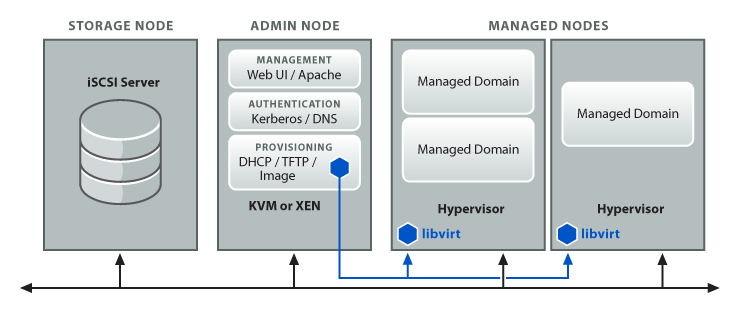
\includegraphics[scale=0.5]{ovirtarch.png}
  \caption{Arquitectura de oVirt}
\label{ovirtarch}
\end{figure}

oVirt consta de una arquitectura relativamente simple, en la cual encontramos al menos \textbf{dos} máquinas:

\begin{itemize}
    \item Un nodo de control: Esta es la máquina donde se instala el oVirt Engine. Desde aquí realizaremos todas tareas de administración y mantenimiento del \emph{datacenter}: despliegue y migración de máquinas virtuales monitorización de los hosts, configuración del almacenamiento, y más.

    \item Hosts de virtualización: Aquí es dónde se ejecutarán las máquinas virtuales. Éstos han de disponer de una CPU con las extensiones de virtualización mencionadas en la sección anterior.
\end{itemize}

La imagen especifica también un tercer nodo: el de almacenamiento. Aquí es donde se guardan tanto las imágenes ISO de instalación de sistemas operativos, como las imágenes de discos duros en uso por las máquinas virtuales. Éste puede ser tanto un host dedicado como en la imagen, o integrarse en el nodo de administración. oVirt soporta diferentes soluciones de almacenamiento en red, como NFS, iSCSI o GlusterFS.\@

Como se ve en la imagen, el nodo de administración y los hosts de virtualización utilizan la API \textbf{libvirt}, para realizar todo el trabajo con máquinas virtuales en materia de creación, arranque y control del almacenamiento. Respecto a la forma de virtualizar, podemos decir que libvirt y KVM virtualizan la máquina virtual por completo, ayudándose de la paravirtualización y las extensiones de virtualización presentes en el procesador.

\section{Requisitos}
\label{subsec:requisitios}

\subsection{Hardware}
\label{subsubsec:hardware}

Los siguientes son las características recomendadas para instalaciones pequeñas y medias, de los diferentes host que forman parte de la arquitectura de oVirt:

\begin{itemize}
\item oVirt Engine
  \begin{itemize}
  \item CPU de dos núcleos.
  \item 4 GB de RAM.\@
  \item 25 GB de espacio libre en el disco duro.
  \item Interfaz de red de 1 Gbps.
  \end{itemize}
\item Hosts de virtualización
  \begin{itemize}
  \item CPU de dos núcleos con extensiones de virtualización (Intel VT-x / AMD-V)
  \item 10 GB de RAM
  \item 10 GB de espacio libre en el disco duro.
  \item Interfaz de red de 1 Gbps.
  \end{itemize}
\end{itemize}

Las máquinas utilizadas para los host de virtualización en éste proyecto, por razones estrictamente monetarias, son un par de Acer Aspire X, con las siguientes especificaciones:

\begin{itemize}
    \item Intel Pentium J29000 (Quad Core, 2,41 GHz)
    \item 4 GB de RAM
    \item 500 GB HD
    \item Interfaz Gigabit Ethernet
\end{itemize}

Obviamente, éstos quedan muy por debajo de los recomendados incluso para instalaciones pequeñas, por lo que éste proyecto no debe considerarse apto para ser llevado a cabo en producción, al menos en su estado actual.

\subsection{Software}
\label{subsubsec:software}

La siguiente lista muestra los sistemas operativos que oVirt soport a la hora de ser virtualizados:

\begin{itemize}
    \item Windows (XP, 7, 8, 2003, 2008, 2012)
    \item RHEL 5, 6 o 7
    \item CentOS 5, 6 o 7
    \item Fedora 16 - 23.
    \item Ubuntu 12.04 + 
    \item openSUSE 12.x+
\end{itemize}


% \chapter{Implementando oVirt}
\label{sec:ovirt}

\section{Instalación del motor}
\label{sec:ovirt_install}

Una vez instalado el sistema operativo en el nodo de control (Fedora, RHEL, o CentOS 7)\footnote{Léase anexo para el proceso de instalación de CentOS}, hace falta actualizar los paquetes del sistema:

\begin{TMterminal}{}{}{Actualizando paquetes}
  yum -y update
\end{TMterminal}

El siguiente paso para instalar oVirt es subscribirnos a su repositorio. Instalar el siguiente RPM es similar a añadir un PPA en distribuciones basadas en Ubuntu en el hecho de que actualizaciones a éste paquete deberían aparecer al hacer más \texttt{yum update} en el futuro.

\begin{TMterminal}{}{}{Instalando oVirt}
  yum install http://plain.resources.ovirt.org/pub/yum-repo/ovirt-release35.rpm
  yum -y install ovirt-engine
\end{TMterminal}

Cuando el paquete se haya instalado, ejecutaremos el instalador del motor, que nos hará una serie de preguntas. El siguiente es un ejemplo del mismo instalador, con las respuestas por defecto envueltas entre corchetes \cite{ovirt}.

\begin{TMterminal}{}{}{Instalación del motor}
  engine-setup
[ INFO  ] Stage: Initializing
   [ INFO  ] Stage: Environment setup
           Configuration files: ['/etc/ovirt-engine-setup.conf.d/10-packaging.conf']
           Log file: /var/log/ovirt-engine/setup/ovirt-engine-setup-20140310163840.log
           Version: otopi-1.2.0_rc2 (otopi-1.2.0-0.7.rc2.fc19)
   [ INFO  ] Stage: Environment packages setup
   [ INFO  ] Stage: Programs detection
   [ INFO  ] Stage: Environment setup
   [ INFO  ] Stage: Environment customization
          
           --== PRODUCT OPTIONS ==--
           --== PACKAGES ==--
          
   [ INFO  ] Checking for product updates...
   [ INFO  ] No product updates found
      
           --== NETWORK CONFIGURATION ==--
          
           Host fully qualified DNS name of this server [server.name]: example.ovirt.org
           Setup can automatically configure the firewall on this system.
           Note: automatic configuration of the firewall may overwrite current settings.
           Do you want Setup to configure the firewall? (Yes, No) [Yes]:
   [ INFO  ] firewalld will be configured as firewall manager.
          
           --== DATABASE CONFIGURATION ==--
          
           Where is the Engine database located? (Local, Remote) [Local]: 
           Setup can configure the local postgresql server automatically for the engine to run. This may conflict with existing applications.
           Would you like Setup to automatically configure postgresql and create Engine database, or prefer to perform that manually? (Automatic, Manual) [Automatic]: 
          
           --== OVIRT ENGINE CONFIGURATION ==--
          
           Application mode (Both, Virt, Gluster) [Both]: 
           Default storage type: (NFS, FC, ISCSI, POSIXFS) [NFS]: 
           Engine admin password: 
           Confirm engine admin password: 
          
           --== PKI CONFIGURATION ==--
          
           Organization name for certificate [ovirt.org]: 
          
           --== APACHE CONFIGURATION ==--
          
           Setup can configure apache to use SSL using a certificate issued from the internal CA.
     
           Do you wish Setup to configure that, or prefer to perform that manually? (Automatic, Manual) [Automatic]: 
           Setup can configure the default page of the web server to present the application home page. This may conflict with existing applications.
           Do you wish to set the application as the default page of the web server? (Yes, No) [Yes]: 
          
           --== SYSTEM CONFIGURATION ==--
          
           Configure WebSocket Proxy on this machine? (Yes, No) [Yes]: 
           Configure an NFS share on this server to be used as an ISO Domain? (Yes, No) [Yes]: 
           Local ISO domain path [/var/lib/exports/iso-20140310143916]: 
           Local ISO domain ACL - note that the default will restrict access to example.ovirt.org only, for security reasons [example.ovirt.org(rw)]: 
           Local ISO domain name [ISO_DOMAIN]: 
          
           --== MISC CONFIGURATION ==--
     
           --== END OF CONFIGURATION ==--

        [ INFO  ] Stage: Setup validation
          
                    --== CONFIGURATION PREVIEW ==--
          
           Engine database name                    : engine
           Engine database secured connection      : False
           Engine database host                    : localhost
           Engine database user name               : engine
           Engine database host name validation    : False
           Engine database port                    : 5432
           NFS setup                               : True
           PKI organization                        : ovirt.org
           Application mode                        : both
           Firewall manager                        : firewalld
           Update Firewall                         : True
           Configure WebSocket Proxy               : True
           Host FQDN                               : example.ovirt.org
           NFS export ACL                          : 0.0.0.0/0.0.0.0(rw)
           NFS mount point                         : /var/lib/exports/iso-20140310143916
           Datacenter storage type                 : nfs
           Configure local Engine database         : True
           Set application as default page         : True
           Configure Apache SSL                    : True
           Please confirm installation settings (OK, Cancel) [OK]:   
   [ INFO  ] Stage: Transaction setup
   [ INFO  ] Stopping engine service
   [ INFO  ] Stopping websocket-proxy service
   [ INFO  ] Stage: Misc configuration
   [ INFO  ] Stage: Package installation
   [ INFO  ] Stage: Misc configuration
   [ INFO  ] Creating PostgreSQL 'engine' database
   [ INFO  ] Configuring PostgreSQL
   [ INFO  ] Creating Engine database schema
   [ INFO  ] Creating CA
   [ INFO  ] Configuring WebSocket Proxy
   [ INFO  ] Generating post install configuration file '/etc/ovirt-engine-setup.conf.d/20-setup-ovirt-post.conf'
   [ INFO  ] Stage: Transaction commit
   [ INFO  ] Stage: Closing up
          
           --== SUMMARY ==--
           `         SSH fingerprint: `<SSH_FINGERPRINT> `         Internal CA: `<CA_FINGERPRINT>
           Web access is enabled at: `             `[`http://example.ovirt.org:80/ovirt-engine`](http://example.ovirt.org:80/ovirt-engine) `             `[`https://example.ovirt.org:443/ovirt-engine`](https://example.ovirt.org:443/ovirt-engine)
           Please use the user "admin" and password specified in order to login into oVirt Engine
          
           --== END OF SUMMARY ==--
          
   [ INFO  ] Starting engine service
   [ INFO  ] Restarting httpd
   [ INFO  ] Restarting nfs services
   [ INFO  ] Generating answer file '/var/lib/ovirt-engine/setup/answers/20140310163837-setup.conf'
   [ INFO  ] Stage: Clean up
           Log file is located at /var/log/ovirt-engine/setup/ovirt-engine-setup-20140310163604.log
   [ INFO  ] Stage: Pre-termination
   [ INFO  ] Stage: Termination
   [ INFO  ] Execution of setup completed successfully
     
     **** Installation completed successfully ******
\end{TMterminal}

\bigskip

\begin{TMterminal}{}{}{Nota}
  Configuraré los \emph{exports} NFS a mano, así que omitiré la parte del instalador que configura un dominio ISO.
\end{TMterminal}

Una vez hecho ésto, ya estaremos listos para acceder a la interfaz web del motor, con la contraseña que le hemos dicho al instalador.

\section{Instalación de los Host}
\label{sec:host_inst}

A la hora de montar los hosts de virtualización, disponemos de varias opciones: podemos instalar el hipervisor propio de oVirt Node, que una vez configurado se añade automáticamente en el motor, o instalar el paquete encima de un CentOS o Fedora ya instalado. Ésta será la opción que documentaré.

Dicho ésto, para instalar el paquete, primero deberíamos asegurarnos que el sistema está actualizado:

\begin{TMterminal}{}{}{Actualizando paquetes}
  yum -y update
\end{TMterminal}

\bigskip

Y instalamos oVirt:

\begin{TMterminal}{}{}{Instalando paquetes}
  yum localinstall http://plain.resources.ovirt.org/pub/yum-repo/ovirt-release36.rpm
\end{TMterminal}

\bigskip

Cuando ya esté instalado, podemos añadirlo manualmente a oVirt, en la pestaña Hosts. Cuando cliquemos en \emph{New}, aparecerá el siguiente diálogo: \clearpage

\begin{figure}[h!]
  \centering
  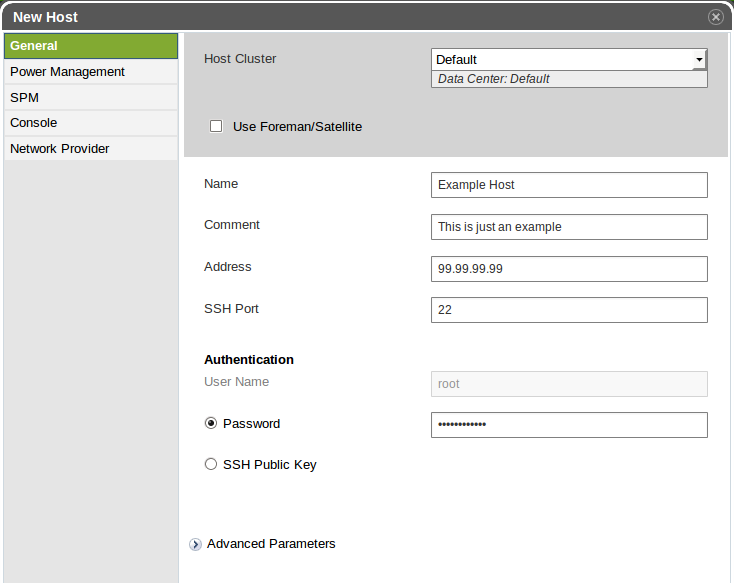
\includegraphics[scale=0.55]{ovirt_hostinst.png}
  \caption{\label{fig:ovirthostinst} Añadiendo el host}
\end{figure}

Una vez añadido, oVirt descargará e instalará ciertos paquetes. Podemos ver el progreso de ésta tarea en la parte inferior de la pantalla, en las pestañas Events y Tasks.

\section{Configuración del almacenamiento}
\label{sec:almacenamiento}

Como ya mencioné cuando describía la arquitectura de oVirt, el almacenamiento viene proporcionado por un sistema en red. Las opciones incluyen soluciones como GlusterFS, iSCSI, o FCP, pero nosotros usaremos NFS.\@ Hay que tener en cuenta, que el tipo de almacenamiento que se use debe coincidir con el tipo por defecto que se seleccionó en el instalador.

Entonces, para configurar los \emph{exports} que usaremos en oVirt, instalamos el servidor, y lo configuramos acordemente \footnote{Ésta configuración sirve sólo de ejemplo: léase la documentación de NFS}:

\begin{TMterminal}{}{}{Configurando NFS}
  yum -y install nfs-utils
  vi /etc/exports
---------------------------
/srv/ovirt/export  *(rw,sync,no_subtree_check,all_squash,anonuid=36,anongid=36)
/srv/ovirt/data    *(rw,sync,no_subtree_check,all_squash,anonuid=36,anongid=36)
/srv/ovirt/iso     *(rw,sync,no_subtree_check,all_squash,anonuid=36,anongid=36)
/usr/ovirt/disks   *(rw,sync,no_subtree_check,all_squash,anonuid=36,anongid=36)
\end{TMterminal}

Una vez hecho ésto, debemos añadirlos en el siguiente orden en la interfaz de administración web:

\begin{enumerate}
    \item Export
    \item Data
    \item iso
\end{enumerate}

\subsection{Cargando las ISOs}
\label{subsec:isos}

Cuando ya tenemos el almacenamiento en red configurado, una particularidad de oVirt es que no podemos abocar directamente al directorio /srv/ovirt/iso las imágenes de instalación, sino que debemos usar la herramienta \texttt{engine-iso-uploader} para subirlas al datacenter, y puedan ser usadas para posteriormente instalar sistemas operativos en las máquinas virtuales. A continuación muestro un ejemplo de dicho comando:

\begin{TMterminal}{}{}{Subiendo ISOs}
  engine-iso-uploader -i nombre_del_dominio_en_ovirt upload imagen.iso
\end{TMterminal}

\subsection{Creando los discos}
\label{subsec:creando_discos}

La creación de los discos puede hacerse tanto al momento de crear la máquina virtual, o cuando el usuario quiera. De todas maneras el proceso es el mismo, detallado en la siguiente captura: 

\begin{figure}[ht!]
  \centering
  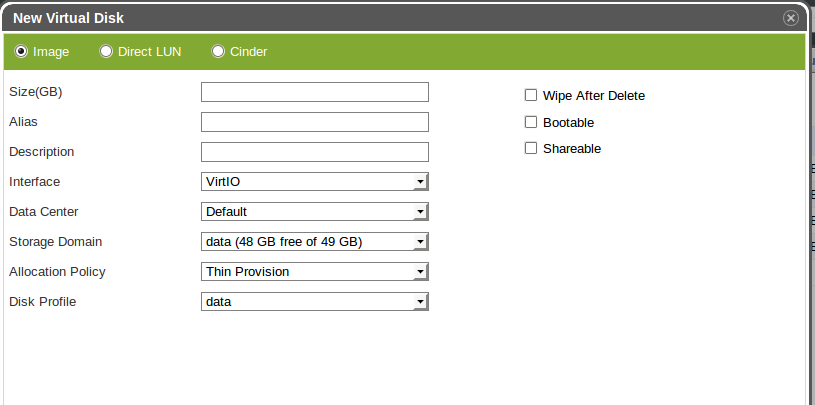
\includegraphics[scale=0.55]{ovirt_newdisk.png}
  \caption{\label{fig:create_disk} Creando discos}
\end{figure}
\clearpage

\subsection{Creando interfaces de red}
\label{subsec:creando_interfaces}

Antes de proceder finalmente a crear una máquina virtual, debemos crear la interfaz de red.

\begin{figure}[ht!]
  \centering
  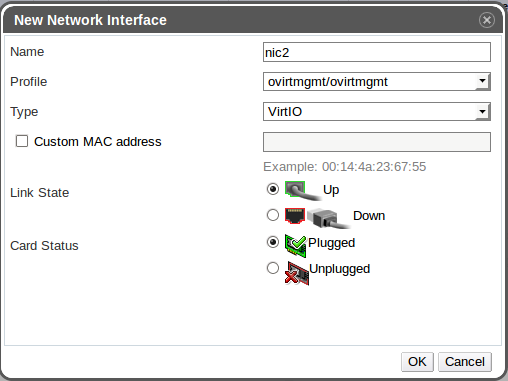
\includegraphics[scale=0.55]{ovirt_newnic.png}
  \caption{\label{fig:create_nic} Creando interfaces de red}
\end{figure}

Acorde a la captura, podemos escoger varios tipos de interfaces de red:

\begin{itemize}
    \item \textbf{VirtIO:\@ }La opción más rápida y ligera, si el sistema virtualizado lo soporta
    \item \textbf{Dos modelos de tarjetas físicas reales: }Su uso supone más \emph{overhead}, ya que tienen que virtualizarse las tarjetas por completo.
    \item \textbf{NIC Passthrough: }Otorga de forma exclusiva una interfaz de red de la máquina anfitriona al sistema virtualizado.
\end{itemize}

\clearpage

\section{Creando máquinas virtuales}
\label{sec:creando_vms}

La creación de las máquinas virtuales es bastante simple. Se puede acceder al diálogo de creación de máquinas virtuales mediante el menú Virtual Machines > New. Las siguientes capturas muestran algunas de las opciones de las que disponemos a la hora de crearlas:

\begin{figure}[ht!]
  \centering
  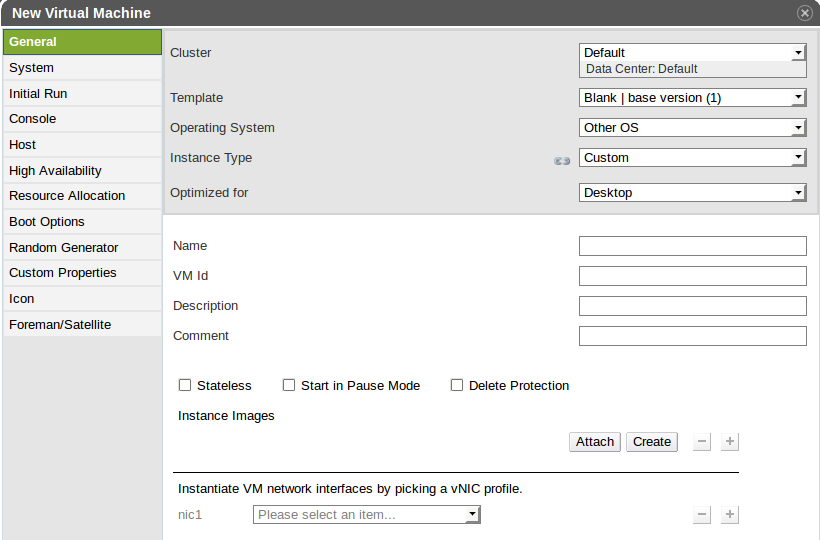
\includegraphics[scale=0.55]{ovirt_newvm.png}
  \caption{\label{fig:create_vms} Creando máquinas virtuales}
\end{figure}

\begin{figure}[ht!]
  \centering
  \frame{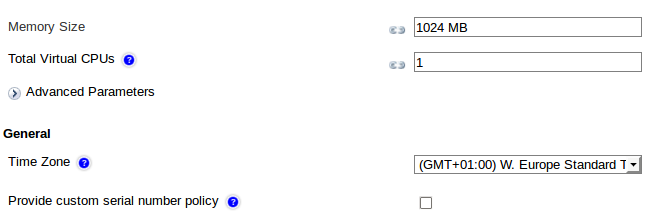
\includegraphics[scale=0.55]{ovirt_vm_system.png}}
  \caption{\label{fig:vmsys} Opciones de sistema}
\end{figure}

\begin{figure}[ht!]
  \centering
  \frame{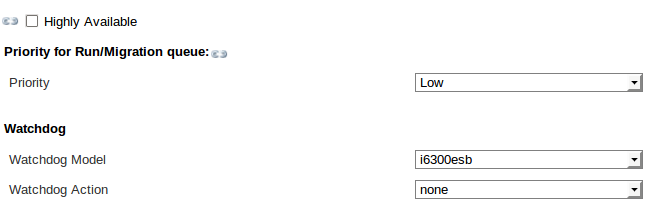
\includegraphics[scale=0.65]{ovirt_vms_ha.png}}
  \caption{\label{fig:vmha} Opciones de alta disponibilidad}
\end{figure}

\begin{figure}[ht!]
  \centering
  \frame{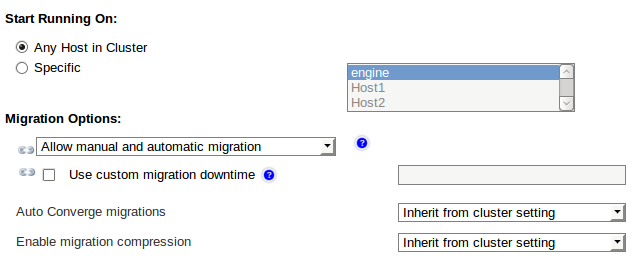
\includegraphics[scale=0.65]{ovirt_vm_host.png}}
  \caption{\label{fig:vmhost} Opciones de host}
\end{figure}

\begin{figure}[ht!]
  \centering
  \frame{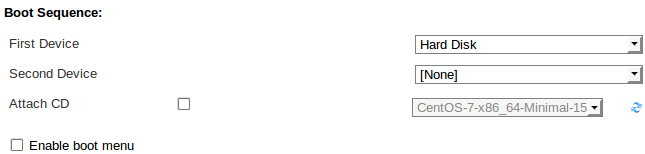
\includegraphics[scale=0.65]{ovirt_vm_boot.png}}
  \caption{\label{fig:vm_boot} Arranque}
\end{figure}

\clearpage
\subsection{oVirt Guest Agent}
\label{subsec:guestagent}

Una vez instaladas las máquinas, debemos instalar el oVirt Guest Agent. Ésta herramienta permite al sistema operativo virtualizado comunicarse con el nodo maestro, ofreciéndole información tal como la dirección IP, el \emph{FQDN} y estadísticas de uso de recursos. El proceso varía dependiendo del sistema operativo, pero a modo de ejemplo, el proceso en Ubuntu es el siguiente:

\begin{enumerate}
\item Editar el fichero \texttt{/etc/apt/sources.list.d/ovirt-guest-agent.list} añadiendo el siguiente contenido:

    \begin{TMterminal}{}{}{/etc/apt/sources.list.d/ovirt-guest-agent.list}
        deb http://download.opensuse.org/repositories/home:/evilissimo:/ubuntu:/14.04/xUbuntu_14.04/ /
    \end{TMterminal}

\item Añadir la \emph{Release key}:

    \begin{TMterminal}{}{}{Añadiendo la release key}
        wget http://download.opensuse.org/repositories/home:/evilissimo:/ubuntu:/14.04/xUbuntu_14.04//Release.key
        sudo apt-key add - < Release.key  
    \end{TMterminal}

\item Y finalmente, actualizamos las listas de software e instalamos el paquete:

    \begin{TMterminal}{}{}{Instalando}
        sudo apt-get update && sudo apt-get install ovirt-guest-agent
    \end{TMterminal}
\end{enumerate}

Una vez esté instalado, el servicio se autoejecutará en cada arranque de la máquina virtual. Si ahora vamos a la interfaz web, deberíamos ver la información de la siguiente manera:

\begin{figure}[ht!]
  \centering
  \hspace*{-1cm}
  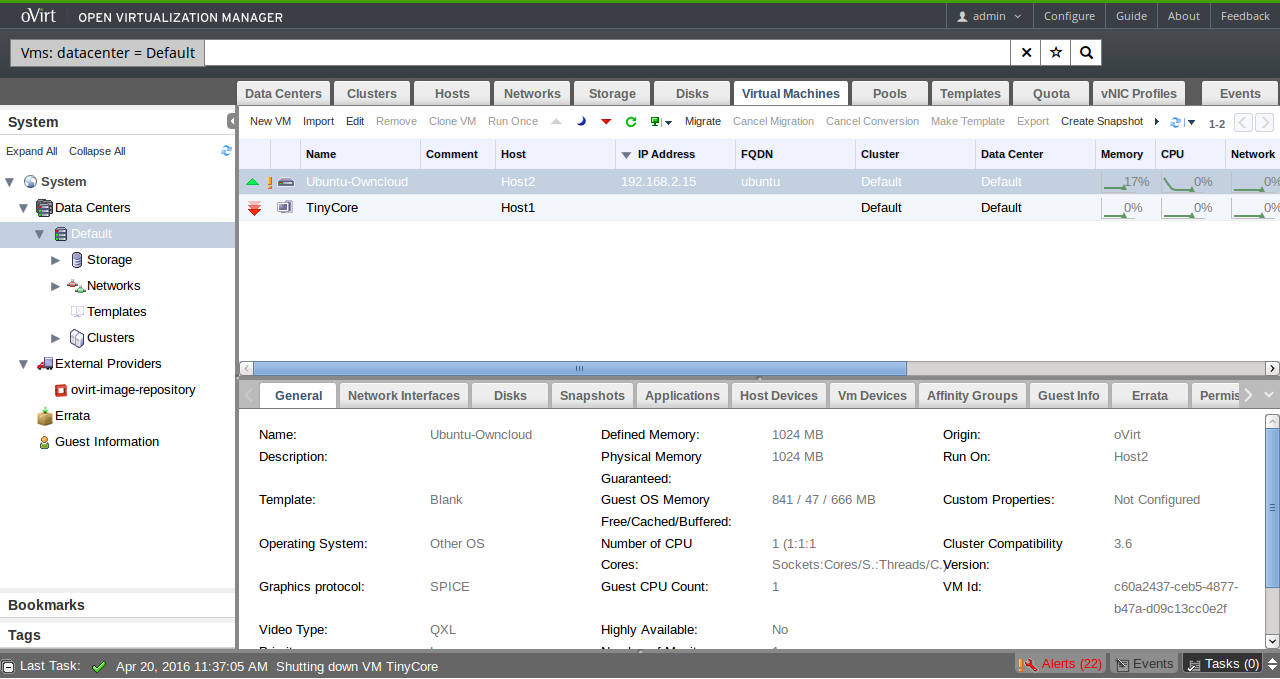
\includegraphics[scale=0.40]{ovirt-vms.png}
  \caption{\label{fig:listado_vms} Lista de máquinas virtuales}
\end{figure}












% \chapter{Conclusiones}
\label{ch:conclusiones}

\section{Objetivos cumplidos}
\label{sec:objetivos}

Durante el transcurso del trabajo, puedo considerar los siguientes objetivos como completados:

\begin{itemize}
    \item Se ha estudiado el uso de la virtualización como herramienta para asegurar servicios.
    \item Se ha estudiado el uso de oVirt como plataforma de gestión del \emph{datacenter}
    \item Assegurar els servidors de l'IES La Bastida a través de la virtualització
    \item Se ha probado la migración de máquinas virtuales, aunque con resultados variados.
    \item Estudiados los mecanismos de copias de seguridad en oVirt.
\end{itemize}

Considerando como el único objetivo que no ha sido completado satisfactoriamente de forma regular es la migración de máquinas virtuales, considero el proyecto un éxito, si menos tomándolo como una prueba de concepto de lo que se puede hacer con oVirt.

Resulta una lástima que hayan cosas que no se hayan podido completar satisfactoriamente, o averiguar por qué fallaban, como en el caso de la migración de máquinas virtuales, pero desde bastante pronto en el proyecto decidí que éste iba a ser más una prueba de concepto que un proyecto a ser implementado tal y como saliera de éste crédito.

\section{Análisis de la planificación y metodología}
\label{sec:plan_metod}

Acercándonos al final del proyecto, considero que la metodología que se decidió seguir este año, realmente no difiere en mucho a como se había hecho en años anteriores. El seguimiento del proyecto fue casi inexistente, cosa que a mí personalmente me llevó a una dinámica que no dista demasiado de cualquier otro proyecto. Por supuesto que adherise rigurosamente al plan de trabajo me correspondía a mí, pero se hubiera agradecido una mayor supervisión, sobretodo en materia de contenido del documento.

\section{Planes de futuro para el proyecto}
\label{sec:futuro}

Una vez concluido el curso, continuaré trabajando en el proyecto, y experimentando con oVirt y otras herramientas, pues el objetivo era encontrar la manera de implementar un sistema alternativo en el IES La Bastida.

Uno de los puntos que más ganas tengo de investigar es el uso de ZFS, recientemente incorporado a Ubuntu 16.04, como sistema de ficheros detrás del almacenamiento en red. En la comparativa de ZFS, btrfs, XFS, ext4 y LVM/KVM realizada por Gionatan Danti \cite{danticomparison}, ZFS sale bastante bien parada de la comparativa con los otros sistemas de ficheros, y ofrece también una serie de características adicionales, como la caché ARC, soporte nativo de \emph{snapshots}, \emph{striping} dinámico, deduplicación de datos, y más.

 Existe también otro punto importante que no he podido tratar en el proyecto por falta de tiempo, el uso de soluciones basadas en \textbf{contenedores}, como Proxmox VE. 

%% \section{Opiniones personales}
%% \label{sec:personal}



% \chapter{Anexo}
\label{ch:anexo}

\section{Instalando CentOS 7}
\label{sec:instalando_centos}

La instalación de CentOS se basa en el instalador Anaconda, que ya viene siendo usado en Red Hat Enterprise Linux y Fedora. Difiere de otros instaladores, en que en lugar de ser lineal, presenta al usuario una \emph{landing screen}, en la cual se encuentran las diferentes preguntas que típicamente se realizan durante una instalación: El particionado de los discos, idioma, distribución de teclado, paquetes a instalar\ldots La siguiente captura muestra dicha pantalla:

\begin{figure}[ht!]
  \centering
  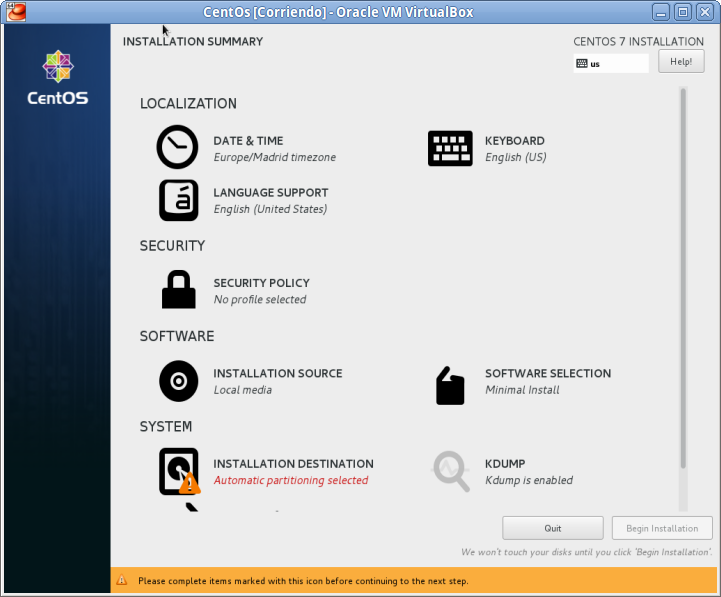
\includegraphics[scale=0.55]{img/anaconda1.png}
  \caption{\label{fig:label} Pantalla principal del instalador Anaconda en CentOS}
\end{figure}

Algunos de los apartados son bastante sencillos y se explican ellos mimsos, así que no incluiré capturas de los mismos. 

\subsection{Localización}
\label{subsec:localizacion}

\subsubsection{Fecha y hora}
\label{subsec:fechahora}

Éste apartado es muy similar al de otros instaladores. Un mapa del planeta aparecerá, dónde podremos seleccionar nuestra ciudad. Acorde a la selección, se ajustará la hora del sistema. Es posible también desactivar NTS, y introducir tanto la fecha como la hora de forma manual.

\subsubsection{Teclado}
\label{subsec:teclado}

Bastante simple también. Aparecerán dos cuadros, uno a la izquierda y otro a la derecha. En la parte inferior del panel izquierdo habrá una lista de botones, que corresponden a Añadir, Quitar, Mover arriba y Mover abajo. Cuando seleccionemos Añadir, aparecerá una lista de idiomas, y las distribuciones de cada idioma una vez se haya seleccionado uno.

En el derecho, simplemente, se podrá probar la distribución de teclado seleccionada.

\subsubsection{Soporte de idiomas}
\label{subsec:soportedeidiomas}

La pantalla de soporte de idiomas es casi exactamente la misma que la primera que encontramos nada más arrancar el instalador, con la única diferencia que en lugar de escoger un único idioma, podemos ir marcando varios, para que luego se instale soporte para todos aquellos idiomas marcados.

\subsection{Discos}
\label{subsec:discos}

Éste es el único apartado \emph{obligatorio} para completar la instalación; todos los demás apartados pueden dejarse con los valores por defecto. Una vez accedemos al apartado, se nos presenta la siguiente pantalla:

\begin{figure}[ht!]
  \centering
  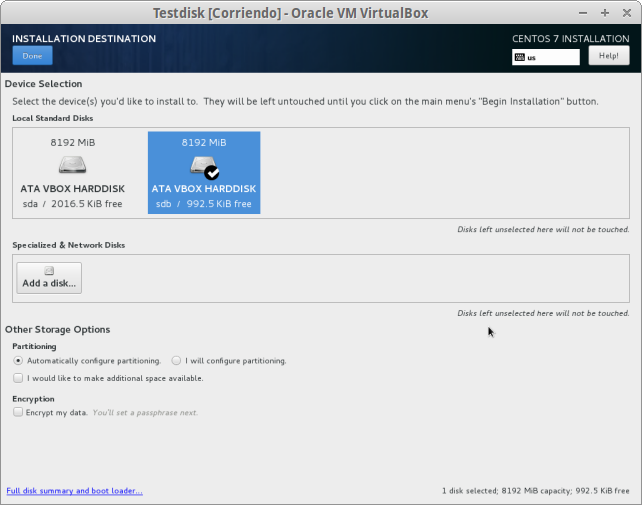
\includegraphics[scale=0.55]{centos-disk1.png}
  \caption{\label{fig:diskselect} Selección de discos}
\end{figure}

\begin{figure}[ht!]
  \centering
  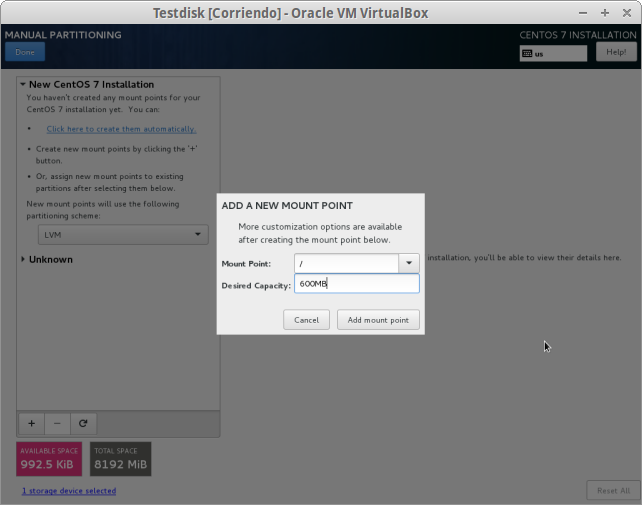
\includegraphics[scale=0.55]{centos-disk2.png}
  \caption{\label{fig:add_mpoint} Añadiendo punto de montaje}
\end{figure}

\begin{figure}[ht!]
  \centering
  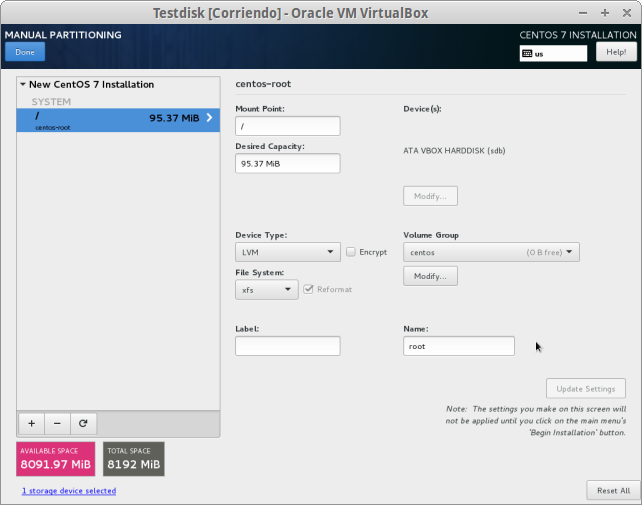
\includegraphics[scale=0.55]{centos-disk3.png}
  \caption{\label{fig:edit_mpoint} Editando punto de montaje}
\end{figure}

\clearpage

\subsection{Continuando la instalación}
\label{subsec:continuando}

Una vez realizado el particionamiento de los discos, la instalación se iniciará, y deberemos editar la contraseña del usuario root, y crear un usuario adicional. 


\section{Trabajando remotamente}
\label{sec:remote}

Dadas las circunstancias del proyecto (No dispongo del hardware físico en el Puig), y que ahora sólo voy aproximadamente ocho horas a la semana a la Bastida, he tenido que buscarme la vida para poder trabajar con las máquinas virtuales en el Puig.

La solución que detallaré ahora a continuación no es muy complicada, pero todo gira en torno a que La Bastida tenga conexión a Internet. Si no puedo llegar hasta su proxy, no puedo trabajar. Una vez dicho esto, lo primero que tengo que hacer para poder acceder a la máquina de la red local de la Bastida donde está instalada la interfaz web del motor, es convertir a mi portátil en un proxy SOCKS.\@Ésto lo puedo hacer mediante el siguiente túnel SSH:

\begin{TMterminal}{}{}{Creando el túnel}
  ssh -D 10080 enrique@ieslabastida.xtec.cat -p 2209
\end{TMterminal}

Mientras la sesión SSH siga activa, mi portátil estará actuando como un proxy SOCKS.\@Si configuro Firefox con dicho proxy como en la siguiente captura: 

\begin{figure}[ht!]
  \centering
  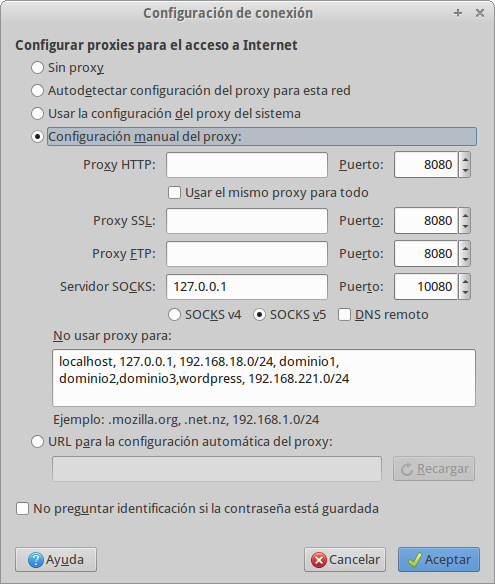
\includegraphics[scale=0.55]{proxyconf.png}
  \caption{\label{fig:Proxy} Configuración del proxy en Firefox}
\end{figure}

Todo el tráfico pasará por el puerto 10080 de mi portátil, que no es ni más ni menos un túnel SSH al Proxy de la Bastida, que atenderá la petición, y me permitirá conectarme al portal de administración.

\subsection{Consola remota mediante el proxy SOCKS}
\label{subsec:consola}

oVirt permite utilizar un cliente de consola remota para conectarse a las máquinas virtuales, y trabajar con el escritorio remoto. Ésto se hace mediante ficheros con extensión $.$vv que permiten a un programa como remote-viewer conectarse. El único problema, es que éste programa no incluye configuración de red, ni la distribución que utilizo (Xubuntu 15.10) incluye configuración global del proxy. La solución a éste problema radica entonces en la librería \textbf{tsocks}, que intercepta todo el tráfico saliente, y lo re-envía a un servidor SOCKS.\@Está pensado para aplicaciones que por defecto no tratan bien con servidores proxy SOCKS.

La siguiente figura muestra la breve configuración (sólo dos líneas) necesarias para hacer que tsocks mande el tráfico por el mismo proxy SOCKS que utilizamos antes:

\begin{TMterminal}{}{}{Configurando tsocks}
  server      = 127.0.0.1
  server_port = 10080
\end{TMterminal}

Una vez editado el fichero de configuración /etc/tsocks, ya podemos ejecutar cualquier programa tal que \texttt{tsocks} \emph{programa}, y todo el tráfico de red que éste genere irá a pasar al servidor SOCKS.









\nocite{*}
\clearpage
\glsaddall
\printglossary[nonumberlist]
\printbibliography[heading=bibintoc]

\end{document}
